\problemname{Deild Goðsagnanna}

The members of the Competitive Programming Association of Iceland play League of Legends quite a lot.
In League of Legends there are two teams, the blue team and the red team, each of which consists of five players.
Each player picks one of the available champions to play for a match before it starts, and no two players can pick the same champion.

Each champion has its weaknesses and strengths, so it is important to pick the right champion that fits well with your teammates' champions and against the opponents' champions.
Therefore it is crucial to pick champions wisely.
In order to prevent the opponents from selecting specific champions, each team may ban several champions from being picked.
Banning a champion means neither team may pick it.

The draft process has the following steps:
\begin{enumerate}
    \item Blue team bans one champion.
    \item Red team bans one champion.
    \item Blue team bans one champion.
    \item Red team bans one champion.
    \item Blue team bans one champion.
    \item Red team bans one champion.
    \item Blue team picks one champion.
    \item Red team picks two champions consecutively.
    \item Blue team picks two champions consecutively.
    \item Red team picks one champion.
    \item Red team bans one champion.
    \item Blue team bans one champion.
    \item Red team bans one champion.
    \item Blue team bans one champion.
    \item Red team picks one champion.
    \item Blue team picks two champions consecutively.
    \item Red team picks one champion.
\end{enumerate}

Originally there were only $20$ champions available,
\footnote{In reality, there were $17$ champions originally, but the draft process required only $16$ champions back then.}
but the developers of the game keep adding more and more champions.
We say two drafts differ if any of their steps differ.
Currently, there are $n$ champions available to choose.
How many different draft processes exist?

Note that it only matters in which step each champion is picked or banned.

Below you can see three images representing three draft processes where the teams picked their champions.
The blue team is on the left and the red team is on the right.
Banned champions appear from left to right.
Picked champions appear from top to bottom.

\begin{figure}[h!]
  \centering
    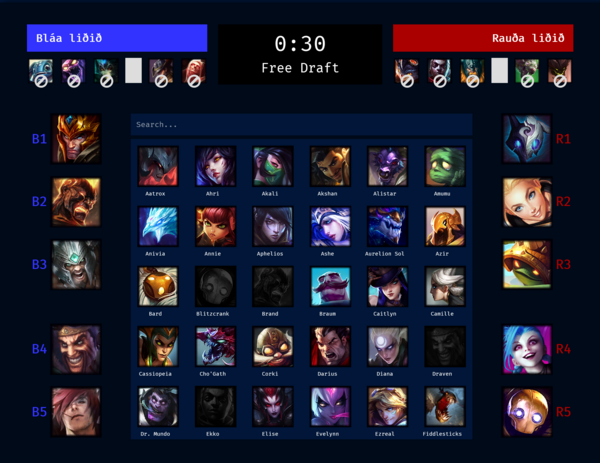
\includegraphics[width=0.8\textwidth]{original_draft.png}
  \caption{Example of a draft process where champions where banned and picked.}
\end{figure}

In the above draft process, the following happens:
\begin{enumerate}
    \item Blue team bans: Fizz.
    \item Red team bans: Rumble.
    \item Blue team bans: Skarner.
    \item Red team bans: Ekko.
    \item Blue team bans: Nami.
    \item Red team bans: Olaf.
    \item Blue team picks: Jarvan IV.
    \item Red team picks: Kindred.
    \item Red team picks: Lux.
    \item Blue team picks: Brand.
    \item Blue team picks: Tryndamere.
    \item Red team picks: Rammus.
    \item Red team bans: Twitch.
    \item Blue team bans: Twisted Fate.
    \item Red team bans: Malphite.
    \item Blue team bans: Vladimir.
    \item Red team picks: Jinx.
    \item Blue team picks: Draven.
    \item Blue team picks: Sett.
    \item Red team picks: Blitzcrank.
\end{enumerate}

\begin{figure}[h!]
  \centering
    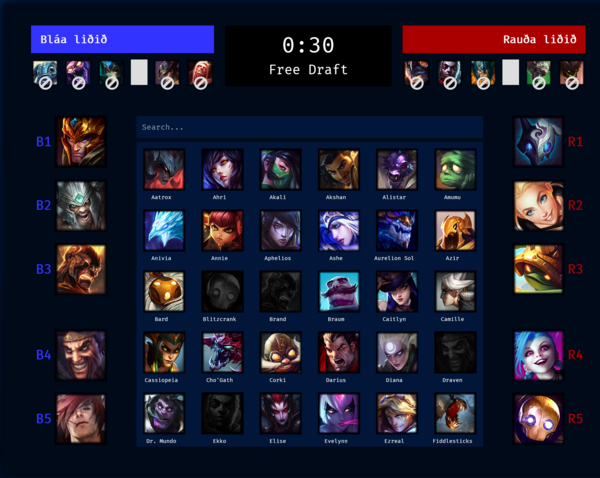
\includegraphics[width=0.8\textwidth]{equivalent_draft.png}
  \caption{This draft process is equivalent to the previous draft process.}
\end{figure}

In the above draft process, the same things happen as in the previous draft process, except that the blue team picks Tryndamere before picking Brand.
Despite that, they are equivalent, since the two picks take place in the same step.

\begin{figure}[h!]
  \centering
    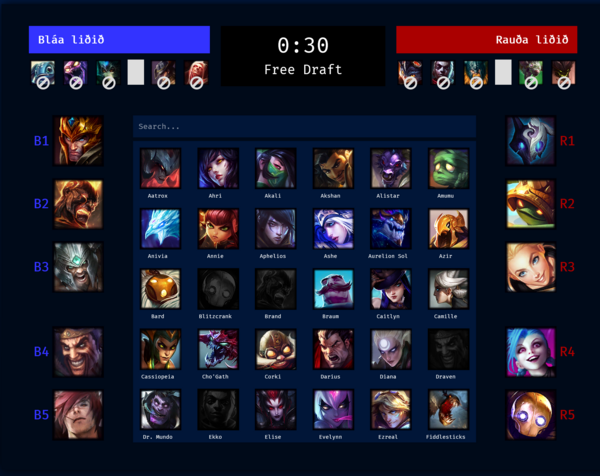
\includegraphics[width=0.8\textwidth]{different_draft.png}
  \caption{This draft process is different from the previous two draft processes.}
\end{figure}

In the above draft process, the same things happen as in the first draft process, except the red team picks Rammus before picking Lux.
These picks take place in different steps, meaning this draft process differs from the previous two.

\section*{Input}
Input consists of one line containing one integer $n$, the number of different available champions in the game.

\section*{Output}
Suppose the number of different draft processes is the integer $k$.
Note that $k$ can be a very large number.
Therefore, you should output one line with one integer, the remainder after dividing $k$ by $1\,000\,000\,007$.

\section*{Scoring}
\begin{tabular}{|l|l|l|}
\hline
Group & Points & Constraints \\ \hline
1     & 30     & $20 \leq n \leq 21$ \\ \hline
2     & 25     & $20 \leq n \leq 100$ \\ \hline
3     & 20     & $20 \leq n \leq 10^{6}$ \\ \hline
4     & 15     & $20 \leq n \leq 10^{9}$ \\ \hline
5     & 10     & $20 \leq n \leq 10^{18}$ \\ \hline
\end{tabular}
